% !TEX root = 0_main.tex
\chapter{Garbled Processor}\label{chap:processor}
Supporting sequential circuits in the \acrshort{gc} protocol enables us to evaluate a general processor as a function in two-party \acrshort{sfe}.
The Boolean circuit of a general processor is a sequential circuit that receives a function (more pressingly the compiled binary code of a function) and data in its memory, then computes the function and writes the result back in the memory.
In this chapter first, we explain the problem of \acrfull{pf-sfe} and how a processor can solve it.
Next, we describe how we used \gls{mips} processor, a simple text-book processor, to resolve the \acrshort{pf-sfe} problem.
Next, we study how a garbled processor can be modified to employ for the \acrshort{sfe} problem as a mean to make it easy for users to develop privacy-preserving applications.
Then, we explain how \gls{arm}, a more sophisticated processor, can be well suited for solving \acrshort{sfe} development if its secure evaluation accompanied by the \gls{skipgate} algorithm.
Versions of \sect{sec:processor-pfsfe} and \sect{sec:processor-pro-pfsfe} of this chapter has been published in 2015 IEEE Symposium on Security and Privacy (S\&P) \cite{songhori2015tinygarble}.
A version of \sect{ssec:processor-mips-sfe-public} of this chapter has been published in 2016 Proceedings of the 53rd Annual Design Automation Conference (DAC) \cite{songhori2016garbledcpu}.


\section{Private Function Evaluation}\label{sec:processor-pfsfe}
Two-party \acrfull{pf-sfe} allows secure computation of a function $g_{Alice}(\cdot)$ held by one party (Alice) operating on another party's data $b_{Bob}$ (Bob) while both the data and the function are kept private.
This setting is in contrast to the usual requirement of \acrshort{sfe} where both parties know the function.
\acrshort{pf-sfe} is especially useful when the function is proprietary or classified.

It is well known that \acrshort{pf-sfe} can be reduced to regular \acrshort{sfe} by securely evaluating a Universal Circuit (\acrshort{uc}) \cite{sander1999non}.
\acrshort{uc} is a Boolean circuit capable of simulating any Boolean circuit (function) $g(\cdot)$ given the description of $g(\cdot)$ as input \cite{valiant1976universal,kolesnikov2008practical}:
$$\acrshort{uc}(b_{Bob},g_{Alice}(\cdot)) = g_{Alice}(b_{Bob}).$$
Secure evaluation of \acrshort{uc} completely hides the functionality and the  topology of the Boolean circuit of $g_{Alice}(\cdot)$.
Subsequent works have shown how to allow \acrshort{pf-sfe} while avoiding the overhead of \acrshort{uc}s \cite{katz2011constant, mohassel2013hide}.

A \acrshort{uc} is similar to a \acrfull{utm} \cite{turing1936computable,herken1995universal} that receives a Turing machine description $g_{Alice}(\cdot)$ and applies it to the input data ($b_{Bob}$) on its tape \cite{davis2001engines}.
One party provides the description, and the other one provides the input data.
After \acrshort{utm} completes the operations, it writes the output $g_{Alice}(b_{Bob})$ on the tape.
A general purpose processor is a special realization of a \acrshort{utm}.
It receives a list of \emph{instructions} $g_{Alice}(\cdot)$ (the compiled binary code of $g_{Alice}(\cdot)$) and applies them to the input data $b_{Bob}$.

\subsection{Arithmetic Logic Unit}\label{ssec:processor-alu}
The core of conventional processors is the Arithmetic Logic Unit (\acrshort{alu}) which receives two \emph{operands} and an \emph{opcode} indicating the desired operation.
\acrshort{alu} supports a set of operations, for example, addition, multiplication, and XOR.
The \acrshort{alu} circuit consists of multiple sub-circuits for these operations and a \acrshort{mux} which selects one of their outputs.
Secure evaluation of an \acrshort{alu}, where the opcode comes from one party and operands come from the other party, keeps the operations private.
Thus, we can think of \acrshort{alu} as an emulator of a simple \acrshort{uc} in which the input function $g_{Alice}(\cdot)$ is limited to a single operation.

One can combine a number of \acrshort{alu}s to make a more comprehensive \acrshort{uc} that can support functions consisting of multiple operations.
Unfortunately, this approach is not practical as the complexity of the circuit grows linearly with the number of operations.
On the other hand, in conventional processors, \acrshort{alu}s are combined with arrays of \acrshort{ff}s, a.k.a., \emph{registers}, to store the intermediate values for supporting functions with an arbitrarily large number of operations.
Since none of the earlier implementations of \acrshort{gc} explicitly supported memory elements such as \acrshort{ff}s, the ways to connect the feedback loop around the \acrshort{alu} were rather limited.
However, an explicit sequential description supported by \gls{tinygarble} allows us to leverage conventional processor architectures.
Therefore, the \gls{tinygarble} methodology not only provides a powerful method for generating compact circuits with a low overhead for \acrshort{sfe} but also paves the way for systematically building scalable sequential circuits used for \acrshort{pf-sfe}.

The idea of using an \acrshort{alu} or a \emph{universal next-instruction circuit} in the \acrshort{gc} protocol can also be found in \cite{liu2014automating}.
The objective of that work was improving the efficiency of \acrshort{sfe} where the function is known by both parties, unlike \acrshort{pf-sfe} where the function is private.
Nonetheless, instead of \acrshort{alu} they eventually decided to use an \emph{instruction-specific circuit} which leaks information about the function but results in less effort for non-private function evaluation.

\subsection{Memory}\label{ssec:processor-mem}
The processor accesses the memory while executing an instruction to read the instruction and data and write the data back.
If the parties evaluate the memory along with the processor in the \acrshort{gc} protocol, they cannot learn about the access patterns of the memory.
On the other hand, if they evaluate the memory separately and outside of \acrshort{gc}, they may learn the access patterns that in turn could reveal information about the function to Bob and the data to Alice.
For example, the instruction read pattern discloses the branching decisions in the function which may leak information about the data.
Because of \gls{tinygarble} sequential methodology, the memory can be easily implemented using \acrshort{mux} and arrays of \acrshort{ff}s.
Thus, it can be included in the processor circuit to be evaluated securely using the \acrshort{gc} protocol.
However, the inclusion of \acrshort{mux}s and \acrshort{ff}s increases the operation time and communication linearly with respect to the memory size.

One alternative approach for hiding memory access patterns is the use of Oblivious Random-Access Machine (\acrshort{oram}) protocols \cite{goldreich1996software} which allow oblivious load/store operations with amortized poly-logarithmic overhead at the expense of increasing the round complexity of the \acrshort{gc} protocol \cite{gordon2012secure,liu2014automating,lu2013garble,gentry2014garbled}.
For the sake of simplicity, we do not use \acrshort{oram} in this thesis.
However, one can simply connect our implementation of \acrshort{pf-sfe} to an \acrshort{oram} to benefit from its lower amortized complexity.
As another alternate, \cite{zahur2013circuit} shows that algorithms can sometimes be rewritten to use data structures such as stacks, queues, or associative maps for which they give compact circuit constructions of poly-logarithmic size.

\section{Garbled Processor for PF-SFE} \label{sec:processor-pro-pfsfe}
\subsection{Global Flow}\label{ssec:processor-mips-flow}
We assume Alice provides the private function $g_{Alice}(\cdot)$ and Bob provides private data $b_{Bob}$.
At the end of the operation, only Bob learns the output $g_{Alice}(b_{Bob})$.
Note that we are not considering the case where both parties learn the output as that would allow AliceS to learn Bob's private data with an identity function ($g\equiv I$).
The protocol is as follows:

\begin{enumerate}
\item
  Alice and Bob agree on an \acrfull{isa}, its implementation (i.e., the processor circuit), the maximum number of sequential cycles, and the configuration of data $b_{Bob}$ in the memory.
\item
  Alice compiles the function $g_{Alice}(\cdot)$ according to the \acrshort{isa}.
  Her input is the compiled binary of the function.
\item
  Bob prepares his input based on the agreed configuration to initialize the processor memory.
\item
  Using any secure \acrshort{gc} framework, Alice garbles the processor circuit for the maximum number of sequential cycles and Bob, after receiving his inputs with \acrshort{ot}, evaluates the garbled processor circuit for the same number of cycles.

\item
  Alice shares the output labels with Bob such that he learns the value of the output $g_{Alice}(b_{Bob})$ stored in memory.
  Alice shares the labels only for the agreed memory locations containing the outputs such that Bob does not learn intermediate values in the memory.
\end{enumerate}

Because of secure evaluation using the \acrshort{gc} protocol in Step 4, no information about values in the circuit leaks except the output.
Without knowing internal values in the processor circuit, none of the parties can distinguish instructions or memory access patterns.
In the following, we demonstrate an implementation of a processor supporting the \gls{mips} \acrshort{isa}, as an example of a garbled processor for securely evaluating private functions.

\subsection{MIPS}\label{ssec:processor-mips}
\gls{mips} is a text-book \acrfull{risc} \acrshort{isa} \cite{kane1992mips}.
The \acrshort{risc} \acrshort{isa} consists of a small set of simplified assembly instructions in contrast to \acrfull{cisc}, e.g., x86 \acrshort{isa}, which includes more complex multi-step instructions \cite{hennessy2012computer}.
We choose a \acrshort{risc} \acrshort{isa} processor instead of \acrshort{cisc} for the following main reasons: (i) lower number of non-XOR gates, (ii) simple and straightforward implementation, and (iii) availability and diversity of open-source implementations.
Moreover, we choose a single-cycle \gls{mips} architecture (i.e., one instruction per sequential cycle).
Other architectures (i.e., multi-cycle and pipelined) increase the performance of the processor by parallelization.
However, the \acrshort{gc} protocol does not benefit from such low-level parallelization.
The only important factor for \acrshort{gc} is the total number of non-XORs which is smaller in the single-cycle \gls{mips}.
We follow the Harvard Architecture which has distinct \acrfull{im} and \acrfull{dm} to separate the parties' inputs.
The \acrshort{im} is a \acrfull{rom} that stores Alice's instructions.
The \acrshort{dm} is a \acrfull{ram} initialized with Bob's input.
The parties' inputs are connected to the initial signals (I) of \acrshort{ff}s in the memories.
Bob's outputs are connected to the outputs (Q) of \acrshort{ff}s in the specified address of the \acrshort{dm}.
The output address in the \acrshort{dm} is part of the agreed memory configuration.

\begin{figure}
\centering
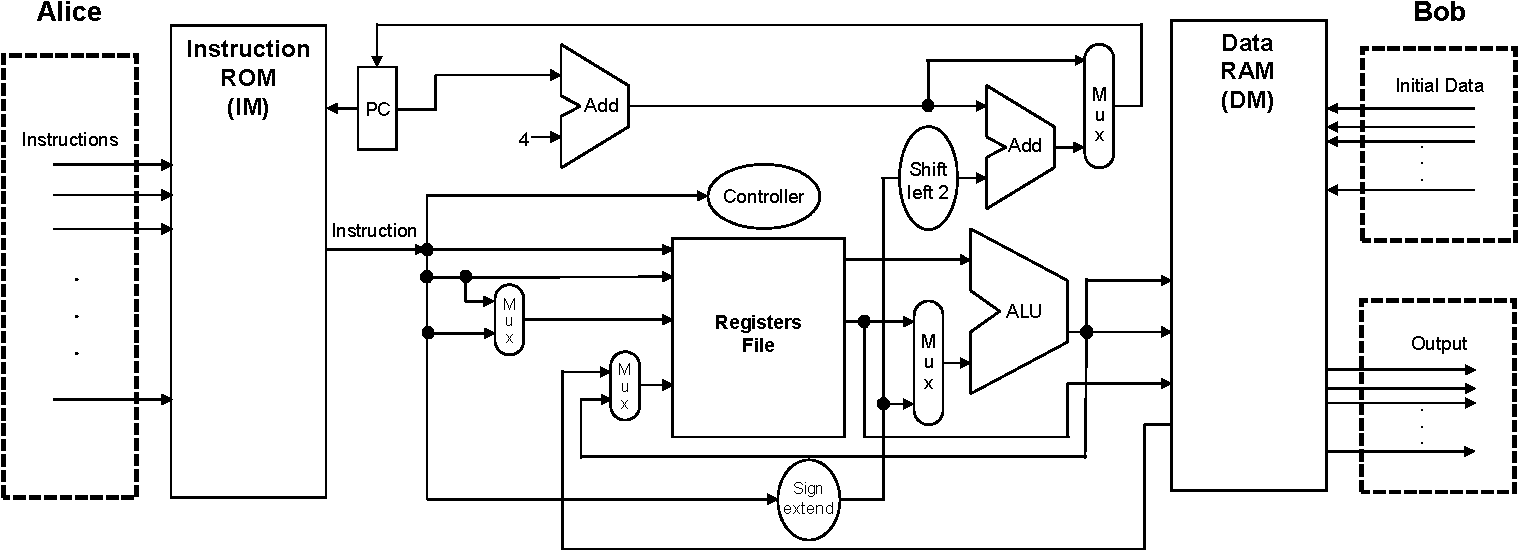
\includegraphics[width=0.95\textwidth]{mips-complex-crop.pdf}
\caption{Lite \gls{mips} architecture.
  Alice's and Bob's inputs and the output are shown.}\label{figure:mips}
\end{figure}

\fig{figure:mips} shows the overall architecture of our 32-bit \gls{mips} processor.
It is based on the Plasma project in opencores \cite{rhoads2006plasma}.
We modified the circuit such that the \acrshort{im} and the \acrshort{dm} are separated.
The original Plasma processor supports all the \gls{mips}~I \acrshort{isa} except unaligned memory access.
In our implementation, we also omit division instructions because of their large overhead.
Any arbitrary function described in \gls{c} language can be easily compiled to \gls{mips}~I assembly code using a cross-platform compiler, e.g., GNU gcc.

In 32-bit \gls{mips}, the \acrfull{pc} is a 32-bit register (array of \acrshort{ff}s) that points to the instruction that the processor is executing at the current cycle.
The processor fetches the instruction from the \acrshort{im} based on the current \acrshort{pc} value.
The \emph{controller} unit is responsible for setting signals to perform the instruction.
In 32-bit \gls{mips}, the \emph{register file} consists of 32 registers of 32-bit each.
In each cycle, at most two registers can be read and at most one register can be written back.
The \acrshort{alu} receives the read register(s) or a sign extended \textit{immediate} as operands.
The \acrshort{alu} also receives an opcode from the controller unit.
The output of the \acrshort{alu} will be either written back to the register file or fed to the \acrshort{dm} as an address for load/store.
The loaded data from the \acrshort{dm} is written back to the register file.
In each cycle, the processor increments the \acrshort{pc} by 4 to point to the next instruction in the \acrshort{im} or changes it according to a branch or jump instruction.

\section{Garbled Processor for SFE}\label{sec:processor-mips-sfe}
In the previous section, we discuss the idea of garbling a processor as a solution for hiding the function in \acrshort{pf-sfe}.
Besides enabling \acrshort{pf-sfe}, another advantage of a garbled processor is usability for non-expert users since it can be programmed using high-level languages, whereas other frameworks for the \acrshort{gc} protocol require tedious Boolean circuit construction.
However, garbling and evaluating the entire processor incurs a tremendous cost compared to \acrshort{sfe} solutions due to stronger privacy requirements in \acrshort{pf-sfe}.

In this section, we expand the garbled processor introduced in \sect{sec:processor-pro-pfsfe} and introduce a framework for secure computation that provides scalable support for generalized \acrshort{sfe}.
The framework provides three options: a high performance with a relaxed privacy setting, the more security-demanding \acrshort{pf-sfe} with a higher cost (similar to the one in \sect{sec:processor-pro-pfsfe}), and a flavor in-between.

To avoid information leakage about the function (i.e., \acrshort{pf-sfe}), we employ the \gls{mips} circuit with its full \acrfull{isa}, which incurs a substantial overhead due to garbling and evaluating of the entire \acrshort{isa}.
We can also compile the function using only a subset of the \acrshort{isa}: restricted \acrshort{isa} (i.e., semi-private function).
A third alternative is public function mode in which the function is compiled using only an application-specific subset of the \acrshort{isa} required for executing the function.
In the following, we discuss these modes of function evaluation and the trade-off between privacy and performance further.

\subsection{Garbled Processor for Public Functions}\label{ssec:processor-mips-sfe-public}
Employ a general-purpose processor supporting its entire \acrshort{isa} for \acrshort{sfe} incurs a significant computation and communication cost.
However, this cost seems unnecessary since both parties know the executed function instructions and they are only interested in learning the output value.
Hence, garbling a limited application-specific \acrshort{isa} for executing each instruction is sufficient to achieve the desired privacy.
To further reduce the \acrshort{isa}, assuming, for example, a function that consists of \numprint{10} instructions, we could theoretically generate $2^{10} -1$ \gls{netlist}s (\gls{netlist}s of \acrshort{isa} with different combinations of the 10 instructions, excluding the \gls{netlist} with zero instructions).
At run-time, one of these \gls{netlist}s is plugged in (garbled and evaluated) at each instruction step depending on the expected instructions.
However, to make it more reasonable (generate fewer \gls{netlist}s), for functions with control flow independent of private data, we know in advance which instruction will be executed at each step.
Thus, we need only the \gls{netlist} of the processor implementing \acrshort{isa} with that specific instruction, restricting the required \gls{netlist}s in this case to \numprint{10}.
For functions with control flow dependent on private data, a simple static analysis can be used to specify the combination of possible instructions at each step, and hence the required \acrshort{isa} \gls{netlist} as proposed in \cite{wang2016secure}.

\subsection{Garbled Processor for Semi-Private Functions}\label{ssec:processor-mips-sfe-semiprivate}
The main cost for garbling a processor with its entire \acrshort{isa} results from garbling circuits for expensive instructions like multiplication and division.
Most compilers can avoid these costly instructions and replace them with cheaper loops of shifts, addition, and subtraction instructions.
These replacements would eliminate the need for the Mult/Div unit in the processor and reduce the cost of garbling per instruction on the one hand.
However, on the other hand, one expensive instruction will be replaced with multiple cheap instructions, thus increasing the total number of instructions.
For example, multiplying two 32-bit numbers with the MULT instruction in \gls{mips} requires \numprint{15} cycles and a circuit of \numprint{13257} non-XOR gates\footnote{XOR gates are evaluated free of cost in \acrshort{gc} according to Free XOR \cite{kolesnikov2008improved}.}, while it requires at least \numprint{31} cycles and a circuit of \numprint{9,676} non-XOR gates when using a conditional loop over an ADD instruction.
We call this mode ``semi-private'' since it only reveals partial information about instructions executed in the program (that the program does not use division/multiplication) and increases the probability of guessing an instruction by reducing the subset of possible instructions (restricted \acrshort{isa}).

\subsection{Garbled Processor for Private Functions} \label{ssec:processor-mips-sfe-private}
In the standard 2-party \acrshort{pf-sfe}, Alice provides the function $g_{Alice}(\cdot)$, Bob provides the input data $b_{Bob}$, and the output is $g_{Alice}(b_{Bob})$.
Similar to \sect{sec:processor-pro-pfsfe}, the garbled processor receives a list of \emph{instructions} of compiled $g_{Alice}(\cdot)$ and applies them to the input data $b_{Bob}$ in memory, and eventually writes the output back to the memory.
To avoid information leakage about the private function, we use a general-purpose processor with its entire \acrshort{isa} (full \acrshort{isa}).

\subsection{Hardware Implementation of Garbled Processor} \label{ssec:processor-hardware}
To the best of our knowledge, the fastest implementation of \acrshort{gc} in hardware was~\cite{jarvinen2010garbled}.
However, their performance is far less than a JustGarble~\cite{bellare2013efficient}, a software implementation.
The reason for this gap is that JustGarble utilizes a more efficient fixed-key \acrshort{aes} for garbling instead of an expensive hash function.
Thus, it is possible that a hardware implementation leveraging the latest \acrshort{gc} optimizations including fixed-key \acrshort{aes} garbling would outperform the software implementation.
Furthermore, a processor is essentially a sequential circuit, and its evaluation requires sequential \acrshort{gc} which no hardware implementation of \acrshort{gc} supports.

We implement our \acrshort{gc} evaluator based on the most recent optimizations listed in \sect{ssec:prelim-imp}.
Its architecture is shown in \fig{fig:evaluator} and consists of:
(1) \acrfull{sscd} memory: a read-only memory that stores the information about gates in the \gls{mips} circuit in \acrshort{sscd} format (see \appx{sec:engine-sscd}).
(2) \acrshort{gc} Label memory: a read-write random-access memory that stores \acrshort{gc} labels of all wires in the corresponding \gls{mips} circuit.
(3) \acrfull{gt} memory: a read-write random-access memory that stores the garbled tables of each non-XOR gate in the \gls{mips} circuit that are generated by Alice (garbler).
(4) Sequential Handler: a controller that supports evaluation of the sequential circuits with the \acrshort{gc} protocol.
(5) Evaluator Core: the implementation of the core functionality of Yao’s \acrshort{gc} protocol's evaluation, its most recent optimizations \cite{kolesnikov2008improved, bellare2013efficient, zahur2015two}, and the sequential garbling presented in \chap{chap:seq}.

As shown in \fig{fig:evaluator}, Bob's input labels in the Label memory are initialized by the \acrshort{ot} protocol with Alice.
The rest of the labels in the Label memory and the Garbled Tables memory are received from Alice.

\begin{figure}
\centering
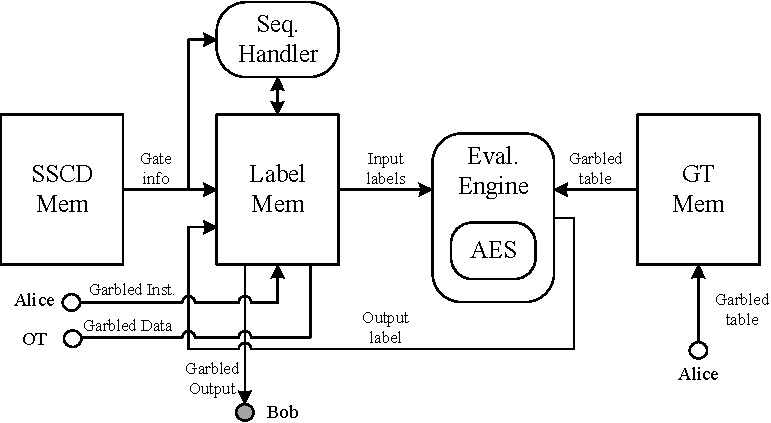
\includegraphics[width=0.8\textwidth]{evaluator-crop.pdf}
\caption{Architecture of our hardware \acrshort{gc} Evaluator.}
\label{fig:evaluator}
\end{figure}

\subsubsection{Pipelined Evaluator Core and Gate Dependency} \label{ssec:processor-hardware-pipeline}
To maximize the performance of our hardware \acrshort{gc} evaluator, we use a 20-stage pipelined \acrshort{aes} implementation \cite{hsing2013tiny} inside our Evaluator Core module.
It increases the throughput of the module by increasing the maximum operating clock frequency of the core.
We also add one stage for the rest of the \acrshort{gc} evaluation functionality.

Due to Free XOR \cite{kolesnikov2008improved}, evaluating an XOR gate requires only XORing the input labels while evaluating a non-XOR gate requires two \acrshort{aes} encryptions \cite{zahur2015two}.
Therefore, the Evaluator Core can finish the evaluation of an XOR gate in one clock cycle of the pipeline.
The different timing for XOR and non-XOR gates introduces a challenge for handling dependencies of gates' inputs and output.
A gate cannot enter the evaluation pipeline if its inputs are another gate's output which is not yet evaluated.
Stalling pipeline is a naive approach for resolving this dependency and degrades the overall performance
To mitigate this, we push XOR gates to the latest empty stage of the pipeline such that the subsequent dependent gates can enter the pipeline as soon as possible.

\subsubsection{Extending Hardware Prototype} \label{ssec:processor-hardware-extend}
In this thesis, we only use on-chip memory for as a proof-of-concept implementation.
However, this prototype can be extended to support interfacing with off-chip memory which would store garbled tables and labels of larger garbled processor circuits and functions.
It can also interface with another \acrshort{fpga} emulator of the garbler which generates the garbled tables and labels and streams them to our evaluator.
A wide range of scenarios is now feasible owing to our current hardware platform and state-of-the-art optimized \acrshort{gc} evaluator.

Such extensions would incur additional area and performance overheads but would allow upscaling of our implementation to support garbled processor circuits and benchmarks in the Gigabytes range.
We emphasize that we provide in this thesis a proof-of-concept prototype to motivate further research in this direction to bring garbled processors some steps closer to the realm of efficient and practical implementations.

\section{ARM2GC: Garbled ARM for SFE}\label{sec:processor-arm}
In this section, we present \gls{arm2gc}, a \acrshort{gc} framework based on a garbled \gls{arm} processor and the \gls{skipgate} algorithm.
The framework aims to simplify the development of privacy-preserving applications while keeping the garbling cost as low as the best optimized garbled circuits.
We first describe the overview of \gls{arm2gc} and its \acrshort{api} for \acrshort{gc} development.
Then, we explain how \gls{arm}'s unique architecture helps to decrease garbling overhead.
Next, the effect of \gls{skipgate} in reducing the garbling cost is discussed.
Finally, we discuss why we do not employ \acrshort{oram} for \gls{arm2gc}.

\subsection{Global Flow}\label{ssec:arm-global}
The \gls{arm2gc} framework allows users to write two-party \acrshort{sfe} program in \gls{c}/C++ (or any language that can be compiled to \gls{arm} binary code).
\fig{fig:frwk_overview} shows the overview of the framework.
The framework benefits from the \gls{skipgate} algorithm to reduce the cost of garbling the \gls{arm} processor.
As described in \chap{chap:skipgate}, the \gls{skipgate} algorithm supports secure evaluation of circuits in the form of $f(a,b,p)$ where $a$ and $b$ are Alice's and Bob's inputs, and $p$ is a public input known to both parties.
In the \gls{arm2gc} framework, the circuit $f(\cdot,\cdot,\cdot)$ is the circuit of \gls{arm} processor and the public input $p$ is the compiled binary code of the user's \acrshort{sfe} program.
To avoid confusion with \gls{arm} circuit, we denote the user's function with $g$.
Similar to other two-party \acrshort{sfe} functions, $g(\cdot,\cdot)$ has two inputs, one from Alice and one from Bob.
The high-level code of $g(\cdot,\cdot)$ is compiled using an \gls{arm} cross-compiler, e.g., gcc-arm-linux-gnueabi.
The compiled binary code of $g(\cdot,\cdot)$ is then passed to the \gls{arm} circuit as the public input $p$.
The parties' private inputs ($a$ and $b$) are passed directly to \gls{arm} circuit: $f(a,b,p)$.
The \gls{skipgate} algorithm then securely evaluate $f(a,b,p)$ by reducing the circuit into the simpler circuit of $f_{p}(a,b) = f(a,b,p)$.
The \gls{arm} circuit computes the function $g(\cdot,\cdot)$ on the private inputs and returns its output: $o = f(a,b,p) = g(a,b)$.

\begin{figure}
\centering
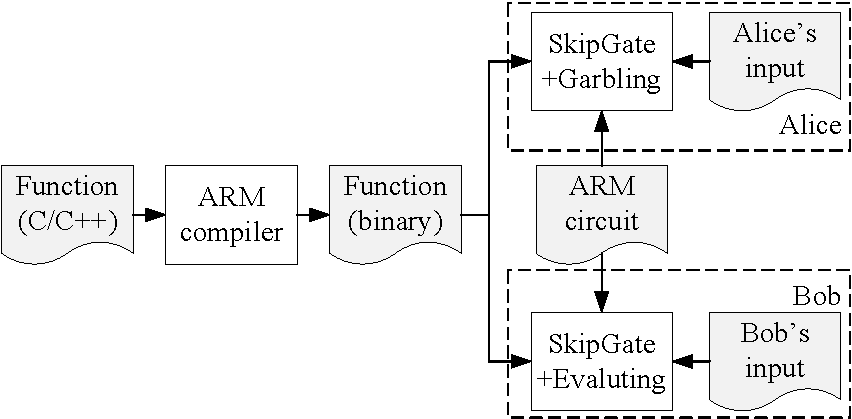
\includegraphics[width=0.7\textwidth]{frwk_overview-crop.pdf}
\caption{Overview of the \gls{arm2gc} framework.}\label{fig:frwk_overview}
\end{figure}

The \gls{arm2gc} framework supports the following \acrshort{api} in \gls{c} language for the user's function $o = g(a,b)$:
\begin{lstlisting}[language=C,basicstyle=\ttfamily,keywordstyle=\color{blue}\ttfamily,stringstyle=\color{red}\ttfamily,commentstyle=\color{CommentColor}\ttfamily]
void gc_main(
  const int *a,// Alice's input
  const int *b,// Bob's input
  int *c) {// output array
  // The user's code goes here.
}
\end{lstlisting}

The entry function, \texttt{gc\_main}, receives three arguments: pointers to Alice's input, Bob's input, and the output.
The circuit of our \gls{arm} processor has five separate memory elements (consisting of \acrshort{ff}s and \acrshort{mux}s) to store: Alice's inputs, Bob's inputs, output, stack, and instructions.
The \acrshort{ff}s in the instruction memory are initialized with the compiled binary code that is known to both parties (the public input $p$).
The flip-flops in Alice's and Bob's memories are initialized with labels corresponding to their private inputs $a$ and $b$ respectively.
The other \acrshort{ff}s in the stack, output, pipeline registers, and the register file are initialized to zero.
The \gls{arm} circuit is garbled using sequential garbling process of \gls{tinygarble} \acrshort{gc} engine (see \appx{chap:engine}) for a pre-specified number of sequential cycles $cc$.

A signal called \textit{terminate} is produced by the \gls{arm} circuit that indicates if \texttt{gc\_main} function is returned.
The signal can be revealed to the parties once in $K$ cycles (predetermined by parties) to reduce the total number of cycles of garbling the \gls{arm} circuit.
For $K=1$, the parties instantly identify the termination, but the exact number of cycles the function evaluated for the given inputs is revealed.
A larger $K$ would reduce this information leakage, but increase the garbling cost.
\appx{chap:engine} provides more details about the support of the terminate signal in \gls{tinygarble} \acrshort{gc} engine.
Eventually, when the function is executed, the parties reveal the content of the output memory to each other to learn output $o = g(a,b)$.

\subsection{ARM as a Garbled Processor}\label{ssec:arm}
In this thesis, we choose \gls{arm} as the garbled processor which is a more ubiquitous and sophisticated processor compared to \gls{mips}.
\gls{arm} has two primary advantages:
(1) Pervasiveness: the compilers and toolsets of \gls{arm} are under constant scrutiny, updating, and probably, more optimized as a result.
(2) Conditional Execution: Designed to improve the performance and code density, conditional execution allows \gls{arm} to execute each instruction only if a specific condition is satisfied~\cite{sloss2004arm}.

\gls{arm} compilers tend to replace conditional branches with conditional instructions to make the flow of the program predictable, and thus, lower the cost of branch mis-prediction.
Similarly, in the garbled processor, the main design effort is to make sure that the flow of the program is predictable so that the next instruction remains public.
Replacing conditional branches with conditional instructions in garbled \gls{arm} generates a code with a predictable flow.
\fig{fig:conditional_exec} shows an example function compiled into assembly with and without the conditional execution.
Moreover, we modify the \gls{arm} controller such that conditional instructions always take the same number of cycles regardless of their condition (taken or not taken).
Otherwise, the program flow will be dependent on the secret condition, and as a result, the program flow itself will become secret which in turn reduces the efficiency of the execution.

\begin{figure}
    \centering
    \begin{subfigure}{0.40\columnwidth}
        \centering
        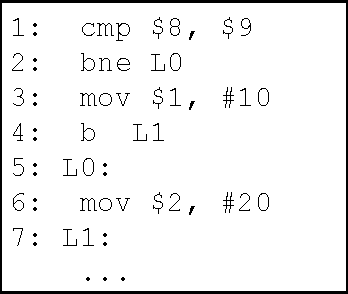
\includegraphics[width=\textwidth]{conditional_exec_wo-crop.pdf}
        \caption{Without Conditional Execution}
    \end{subfigure}
    ~
    \begin{subfigure}{0.40\columnwidth}
        \centering
        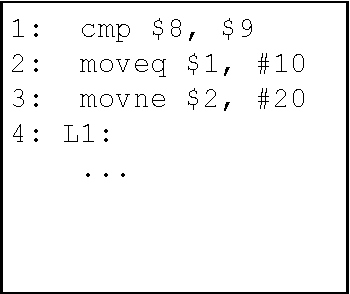
\includegraphics[width=\textwidth]{conditional_exec_w-crop.pdf}
        \caption{With Conditional Execution}
    \end{subfigure}
    \caption{An example code showing how conditional execution in \gls{arm} can reduce the code size and make the program flow predictable.}\label{fig:conditional_exec}
\end{figure}

We modify and remove a few features from the \gls{arm} processor like interrupts, co-processors, and performance-related components including cache and pipeline.
The last group does not bring any performance advantages in the \acrshort{gc} protocol, as the circuit is garbled/evaluated gate by gate (serially).
Note that unlike in hardware, the performance of \acrshort{gc} does not increase by parallelizing gates in the circuit.
In the \acrshort{gc} protocol, the total number of non-XOR gates is the only factor affecting the performance, not the circuit's topology.

Implementation of the \gls{arm} processor results in a complex and large circuit (containing almost five times more gates than the \gls{mips} processor).
Thus, using \gls{arm} instead of \gls{mips} would incur even a higher cost.
However, the majority of the components of the \gls{arm} processor remain idle during  execution of an instruction.
In the next section, we describe how \gls{skipgate} utilizes this characteristic to minimize the cost of garbling the \gls{arm} processor.

\subsection{How {SkipGate} Helps}
As explained above, we initialize the instruction memory of the \gls{arm} with public values.
Therefore, if the program counter (the address of the next instruction) is public, the next instruction becomes public as well.
As a result, the control path also becomes public, and \gls{skipgate} can easily detect the idle components to mark them for skipping.
Moreover, due to \gls{skipgate}, the gates of the active components that are only transporting data between memory, register file, and \acrshort{alu} act as wires and do not incur any cost.
According to \gls{skipgate}'s notation, the \gls{arm} Boolean circuit is a 3-input function $o = f(a,b,p)$ where $p$ is equal to the compiled binary code of $g(a,b)$ and $a$ and $b$ are the parties' private inputs.
\gls{skipgate} reduces the \gls{arm} circuit into a smaller circuit of $o = f_p(a,b)$ where $f_p$ can perform the exact operation required in the function $g(\cdot,\cdot)$.
Therefore, the main garbling cost is paid only for the actual computation of the secret values.
As explained in the previous section, \gls{skipgate} performs these optimizations at the gate-level, in contrast to instruction-level of the approaches in \sect{sec:processor-mips-sfe} and \cite{wang2016secure}.

\subsection{Why not Sub-linear ORAM?}
As mentioned in \sect{ssec:arm-global}, we use an array of \acrshort{mux}s and \acrshort{ff}s to implement the register file in \gls{arm} circuit.
This structure means that the cost of accessing the register file, when performed obliviously, is linear with respect to its size.
One natural question would be why we did not employ \acrfull{oram} that enables oblivious access to memories in the \acrshort{gc} protocol with sub-linear cost~\cite{wang2014scoram, zahur2016revisit}.
The reason is that, in most cases, the access to the register file is not required to be oblivious.
Since the instructions come from the publicly known instruction memory, both parties know which register of the register file is read or written.
The \gls{skipgate} algorithm utilizes this to skip garbling of the gates in the \acrshort{mux}s of the register file.
Thus, no cost is required for such accesses.
With \acrshort{oram}, all the accesses to the register file would be the costly oblivious access of \acrshort{oram}.

In rare occasions where two or more instructions should be garbled at a time, accessing a register would not be free using \acrshort{mux}s and \gls{skipgate}.
These cases only happen when \gls{arm} compiler fails to replace a conditional branch on a secret value with conditional instructions.
The user can typically alter the program in a way that the compiler avoids such branches and replaces it with conditional instructions instead.
However, in these cases, the \gls{skipgate} algorithm removes most of the gates in the register file.
Since the cost of fetching instructions remains smaller than that of break-even points of sub-linear \acrshort{oram}s, using \acrshort{oram} would not improve the efficiency for this case either.

\begin{figure}
\centering
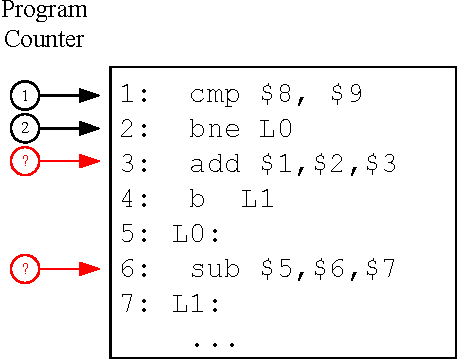
\includegraphics[width=0.5\textwidth]{branch-crop.pdf}
\caption{In case of compiler failure to replace a secret branch with conditional instructions, the parties do not know which instruction is executed after the branch.
Thus, the instruction becomes secret.}
\label{fig:branch}
\end{figure}

\fig{fig:branch} shows an example where after execution of a branch on a secret value, the next instruction becomes secret and unknown to parties.
In this example, the program counter can be either 3 or 6 depending on the outcome of the comparison in Line 1.
Thus, two instructions \texttt{add \$1, \$2, \$3} (\texttt{\$3 = \$1 + \$2}) and \texttt{sub \$5, \$6, \$7} (\texttt{\$5 = \$6 - \$7}) have to be garbled/evaluated at the same time.
For fetching the second register in instruction from the register file, we only have two choices: \texttt{\$2} and \texttt{\$6}.
This limited choice means that, instead of having a complete oblivious access to the register file with 16 options, we only have to select obliviously between 2 of the 16 registers.
This cost is far less than 1-out-of-16 oblivious access.
The cost of oblivious access using \acrshort{mux}s and \gls{skipgate} to a \textit{subset} of memory is equal to an oblivious access to a memory with the size of the subset.

\begin{figure}
\centering
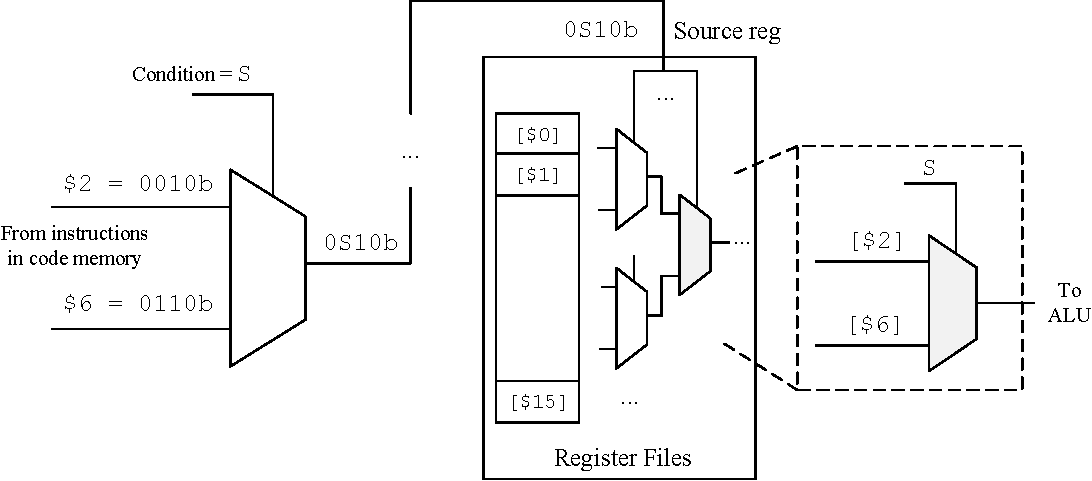
\includegraphics[width=0.9\textwidth]{registers-crop.pdf}
\caption{Bit-precise details of how source register is fetched while executing two instructions \texttt{add \$1, \$2, \$3} and \texttt{sub \$5, \$6, \$7} at the same time after a branch on a secret condition value \texttt{S}.}
\label{fig:registers}
\end{figure}

\fig{fig:registers} illustrates the details of the above example where bit \texttt{S} is the secret bit that separates the branches of computation that each is leading into a different instruction.
The address of the source register is computed by a \acrshort{mux} over the two options in the two instructions: \acrshort{mux}(\texttt{\$2, \$6, S}) = \acrshort{mux}(\texttt{0010b, 0110b, S}) = \texttt{0S10b}.
The most and least significant bits are, in either case, zero, and thus it will remain zero in the output.
The bit 1 is one in both cases and remains one.
The bit 2 is zero if \texttt{S==0} and is one if \texttt{S==1}, and thus this bit is equal to \texttt{S}.
Now, let us look at the \acrshort{mux}s in the registers files that fetch the source register.
The \acrshort{mux}s connected to the known bit can be evaluated separately by both parties, and thus \gls{skipgate} will avoid garbling/evaluating them.
Within the \acrshort{mux}s connected to \texttt{S}, only the one that selects between \texttt{[\$2]} and \texttt{[\$6]} remains for garbling, and \gls{skipgate} will skip the rest due to non-positive fanout.

% why not \acrshort{oram} for code and data memory
The rationale for using an array of \acrshort{mux}s in the register file also applies to the code, data, and stack memories where the access is almost always public and known to both parties.
In the worst case, only a subset of memory is accessed obliviously, thus making the cost of memory access below the threshold of switching to \acrshort{oram}s.

% Research question
The mixture of the \gls{skipgate} algorithm and garbled processor introduces an unusual use-case for oblivious memory where oblivious access is performed only on a varying subset of the memory.
The subset can be different from one access to the other.
The current sub-linear \acrshort{oram} protocols cannot address this scenario efficiently.
Thus, an interesting research question is raised:

\textbf{Is it possible to \textit{obliviously} access (read/write) a varying subset of the memory with a \textit{sub-linear} cost in terms of the subset size?}
